\documentclass[oneside,12pt,a4paper,final]{book} %opt: draft/final
\usepackage[czech]{babel}
\usepackage[utf8]{inputenc}
\usepackage{graphicx} % support the \includegraphics command and options
\usepackage{hyperref} % links in \tableofcontents
\usepackage{minted} % syntax highlighter
\usepackage{pdfpages}
\usepackage{textcomp}
\usepackage{float} % figure [H]
\usepackage{pgfplots} % tikzpicture
\usepackage{amsmath} % linebreaks in math mode
\usepackage{dirtree} % struktura slozek
\usepackage{makeidx} % rejstrik

\makeindex

\hoffset=0.5cm % posune stranku ->

\hypersetup{
	colorlinks,
	citecolor=black, %blue
	filecolor=black,
	linkcolor=black, %red
	urlcolor=black %blue
}
\addto\captionsczech{\renewcommand{\chaptername}{}} %remove "chapter" word

\pgfplotsset{major grid style={lightgray!50!white}}
\pgfplotsset{soldot/.style={color=blue,only marks,mark=*}}
\pgfplotsset{holdot/.style={color=blue,fill=white,only marks,mark=*}}

\makeatletter
\newcommand{\tocfill}{\cleaders\hbox{$\m@th \mkern\@dotsep mu . \mkern\@dotsep mu$}\hfill}
\makeatother
\newcommand{\abbrlabel}[1]{\makebox[6cm][l]{\textbf{#1}\ \tocfill}}
\newenvironment{abbreviations}{\begin{list}{}{\renewcommand{\makelabel}{\abbrlabel}%
        \setlength{\labelwidth}{6cm}\setlength{\leftmargin}{\labelwidth+\labelsep}%
                                              \setlength{\itemsep}{0pt}}}{\end{list}}

\newcommand{\namesig}[2][5cm]{%
  \begin{tabular}{@{}p{#1}@{}}
    #2 \\[5\normalbaselineskip] \dotfill \\[0pt]
    {\small \textit{Podpis}}
  \end{tabular}
}

\interfootnotelinepenalty=10000 %BRUTAL!

\begin{document}

%%% TITLE
\pagestyle{empty}
\begin{titlepage}
\noindent
\begin{center}
	{\LARGE ZÁPADOČESKÁ UNIVERZITA V~PLZNI} \\[0.1cm]
	{\LARGE FAKULTA ELEKTROTECHNICKÁ} \\[0.4cm]
	{\Large\sc Katedra elektroenergetiky a~ekologie} \\
	\vspace{5cm}
	{\Huge\sc Bakalářská práce} \\
	\vspace{1cm}
	{\large Návrh a realizace real-time komunikace pro senzorickou síť\\s webovou řídicí aplikací\\}
	\vspace{1cm}
	{\large Design and Implementation of Real-time Communication for Sensory Network with Website Based Control Application}
\end{center}
\vfill
Autor práce: Martin Zlámal\\
Vedoucí práce: Ing. Petr KRIST, Ph.D. \hfill Plzeň 2015
\end{titlepage}

\pagestyle{plain}
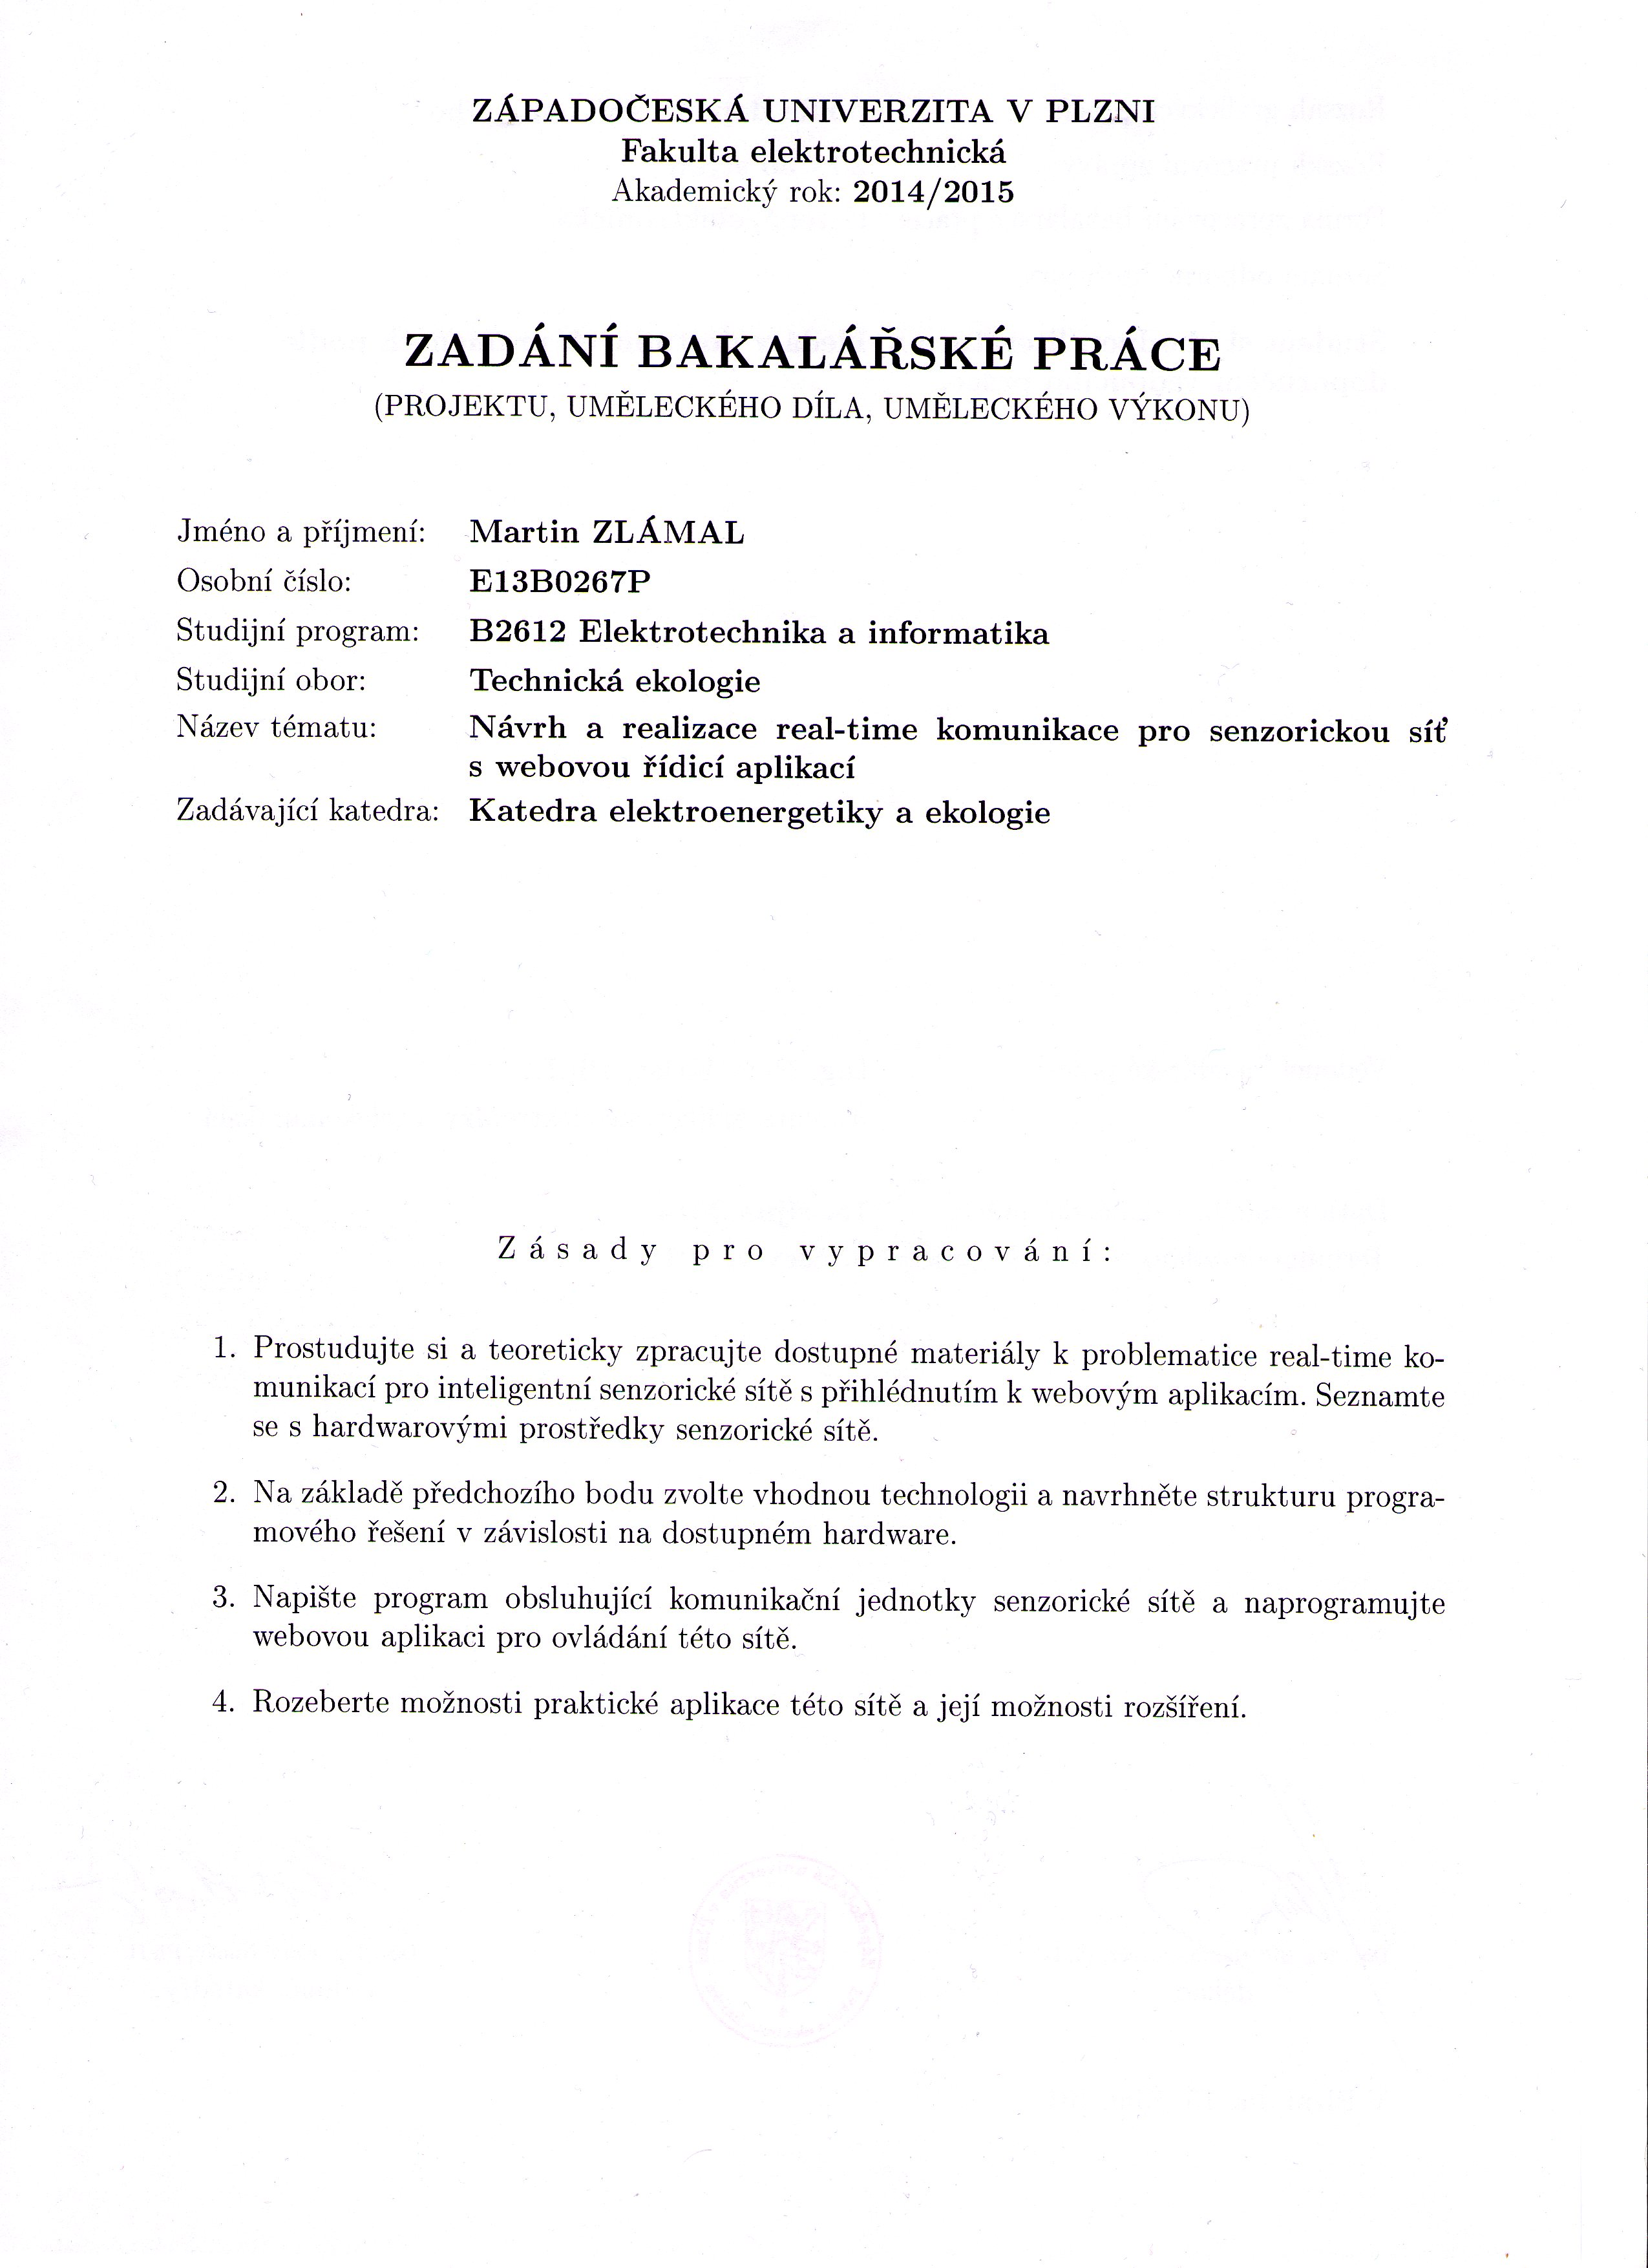
\includepdf[pages={1}]{img/zadani1.jpg}
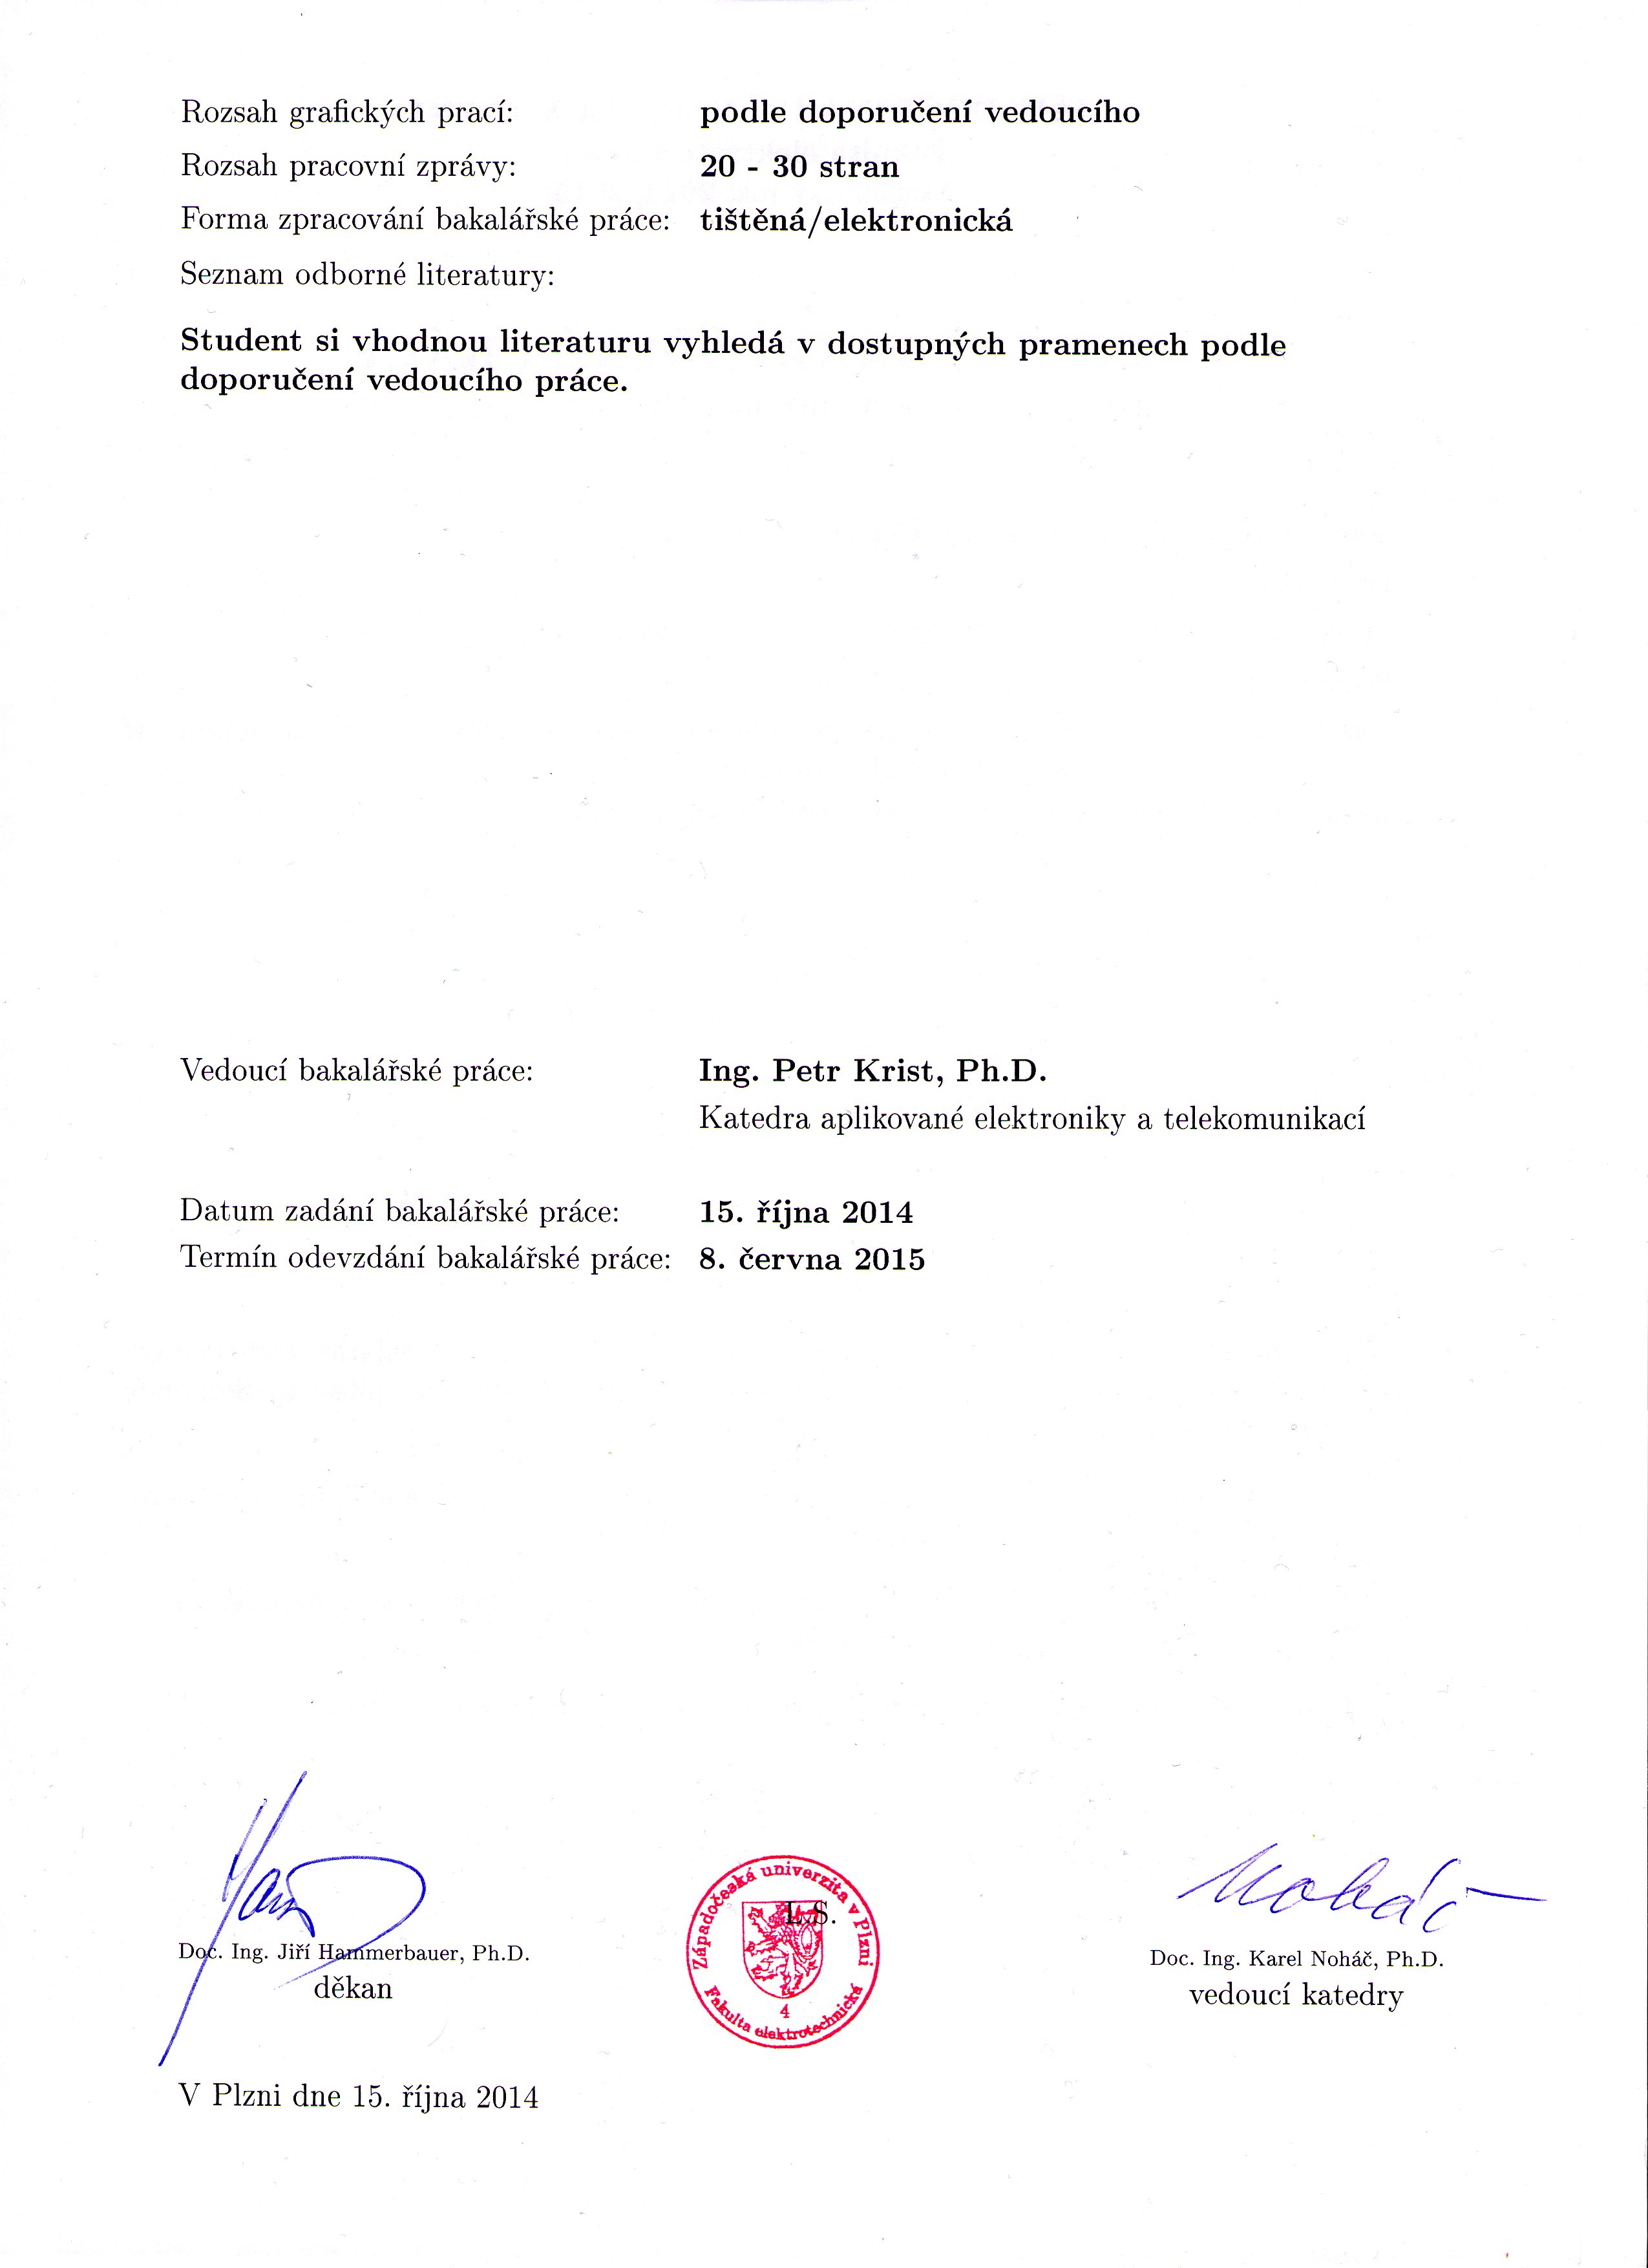
\includepdf[pages={1}]{img/zadani2.jpg}
\chapter*{Abstrakt}
Text abstraktu v češtině...

\vfill
\section*{Klíčová slova}
Ethernet, Expres.js, Node.js, Procesor, Redis, RESP, TCP, UDP, Websocket
\pagenumbering{roman}
\chapter*{Abstract}
Text abstraktu v angličtině...

\vfill
\section*{Key Words}
Ethernet, Expres.js, Node.js, Procesor, Redis, RESP, TCP, UDP, Websocket
\chapter*{Prohlášení}
Předkládám tímto k~posouzení a obhajobě bakalářskou práci, zpracovanou na závěr studia na Fakultě elektrotechnické Západočeské univerzity v~Plzni.

Prohlašuji, že jsem svou závěrečnou práci vypracoval samostatně pod vedením vedoucího bakalářské práce a s~použitím odborné literatury a dalších informačních zdrojů, které jsou všechny citovány v~práci a uvedeny v~seznamu literatury na konci práce. Jako autor uvedené bakalářské práce dále prohlašuji, že v~souvislosti s~vytvořením této závěrečné práce jsem neporušil autorská práva třetích osob, zejména jsem nezasáhl nedovoleným způsobem do cizích autorských práv osobnostních a jsem si plně vědom následků po\-ru\-še\-ní ustanovení § 11 a následujících autorského zákona č. 121/2000 Sb., včetně možných trestněprávních důsledků vyplývajících z~ustanovení § 270 trestního zákona č. 40/2009 Sb.
\chapter*{Poděkování}
Děkuji vedoucímu této bakalářské práce Ing. Petru Kristovi, Ph.D. za jeho čas věnovaný této práci při konzultacích a za motivaci, která mě nutila posouvat své hranice stále dál. Mé poděkování patří také společnosti UNIOSO s.r.o. za cenné připomínky při návrhu celého systému a za poskytnutí vývojových desek značky STMicroelecronics, bez kterých by vytvoření této práce nikdy nebylo možné.


\tableofcontents
\cleardoublepage
\phantomsection
\addcontentsline{toc}{chapter}{\listfigurename}
\listoffigures


\chapter*{Seznam symbolů a zkratek}
\addcontentsline{toc}{chapter}{Seznam symbolů a zkratek}
\noindent
\begin{abbreviations}
\item[ADC]		Analog-to-Digital Converter
\item[AJAX]		Asynchronous JavaScript and XML
\item[AJAJ]		Asynchronous JavaScript and JSON
\item[BGA]		Ball Grid Array
\item[BSP]		Board Support Package
\item[CAN]		Controller Area Network
\item[CPU]		Central Processing Unit
\item[CRLF]		Carriage Return Line Feed
\item[DHCP]		Dynamic Host Configuration Protocol
\item[EDA]		Event-Driven Architecture
\item[EJS]		Embedded JavaScript
\item[HAL]		Hardware Abstraction Layer
\item[HTTP]		Hypertext Transfer Protocol
\item[ICMP]		Internet Control Message Protocol
\item[I/O]		Input/Output
\item[IoT]		Internet of Things
\item[IP]		Internet Protocol
\item[JS]		JavaScript
\item[JSON]		JavaScript Object Notation
\item[JSONP]	JSON with padding
\item[LED]		Light-Emitting Diode
\item[MAC]		Media Access Control
\item[MVC]		Model View Controller
\item[NPM]		Node Package Manager
\item[OS]		Operating System
\item[PWM]		Pulse Width Modulation
\item[RAM]		Random-Access Memory
\item[RESP]		Redis Serialization Protocol
\item[RFC]		Request for Comments
\item[RTT]		Round Trip Time
\item[SMA]		Simple Moving Average
\item[TCP]		Transmission Control Protocol
\item[TED]		Technology, Entertainment, Design
\item[UDP]		User Datagram Protocol
\item[UTP]		Unshielded Twisted Pair
\item[UFBGA]	Ultra Fine BGA
\item[XHR]		XMLHttpRequest
\item[XML]		Extensible Markup Language
\end{abbreviations}



\chapter{Úvod}
\pagenumbering{arabic}
Cílem této práce je navrhnout komunikaci pro senzorickou síť s přihlédnutím k tomu, že by tato síť měla být ovladatelná v reálném čase z webové řídící aplikace. Toto je velmi zásadní požadavek pro budoucí realizaci, protože z hlediska elektronických systémů je real-time komunikaci možné realizovat pomocí protokolů k tomu určených, které vymezují přenos dat do přesně definovaných časových slotů(Ethernet Powerlink, Time-triggered CAN, FlexRay). U webových aplikací žádný takový prvek neexistuje a webová řídicí aplikace se tak stává limitujícím prvkem celé sítě. Existují však metody, které se real-time komunikaci resp. rychlé komunikaci, jak je real-time u webových aplikací všeobecně chápán, mohou velmi přiblížit. V roce 2011 bylo vydáno RFC 6455 \cite{rfc6455}, které zastřešuje nový protokol websocket, který umožňuje propojení serveru a klientské části aplikace socketem a je tak možné přenášet informace velmi vysokou rychlostí, což doposud nebylo prakticky téměř možné realizovat.

V následující části práce bude rozebrána problematika komunikace senzorické sítě s webovou řídicí aplikací, ze které vyplyne, že nejvhodnějším řešením je naprogramovat jednotlivé členy senzorické sítě co nejvíce ní\-zko\-ú\-rov\-ňo\-vě, následně je propojit s řídicím serverem, na kterém poběží Node.js real-time server (asynchronní single-thread) pro zpracovávání požadavků a zároveň zde poběží server pro webovou aplikaci, která bude využívat websocket protokolu coby nástroje pro komunikaci s tímto serverem. Zároveň je tato senzorická síť uváděna na příkladu administrativní budovy resp. jakéhokoliv objektu kde se běžně pohybují lidé a využívají konvenční elektroinstalaci, tzn. například domácí objekty, popřípadě jiné objekty podobného charakteru kde má využití této sítě praktický přínos.
\chapter{Real-time komunikace}
Real-time komunikace představuje významný prvek v aplikacích, kde je zapotřebí velmi rychlých reakcí systému. Zpravidla se za real-time aplikaci považuje systém, který řeší časové korekce posílaných signálů a tedy vzájemnou časovou synchronizaci vysílače a přijímače. Obecně lze však za real-time aplikaci uvažovat systém, který reaguje na požadavky bez zbytečného dopravního zpoždění, které je například u webových aplikací naprosto běžné. Předejít však dopravnímu zpoždění u webových aplikací není možné. Důvod je prostý. Webová aplikace musí být dostupná pro všechny uživatele na celém světě a z toho plyne, že každý uživatel je na jiném geografickém místě a čas potřebný k dostání informace ke koncovým uživatelům není stejný. Tento problém lze částečně vyřešit distribuovaným systémem, kdy se servery přibližují uživatelům, což prakticky dělají například streamovací portály jako je YouTube. Toto řešení má svá omezení a proto druhým způsobem, jak ušetřit čas při komunikaci s koncovým prvkem, je zjednodušit komunikační protokol, nebo se omezit na co nejméně zbytečné režie a to i za tu cenu, že nedojde ke stoprocentnímu přenosu informace.

\section{Hardwarové prostředky senzorické sítě}
Hardwarové prostředky této sítě nejsou v současné chvíli nijak přesně definovány. Je tedy možné síť navrhnout libovolným způsobem. Vzhledem ke komplikovanosti celé problematiky bude tato síť striktně metalická paketová. Taková síť se tedy skládá v nejmenší konfiguraci pouze z koncového členu a serveru. S narůstajícím počtem koncových členů je zapotřebí síť patřičně rozšiřovat. Výhodou tohoto systému je fakt, že se daná síť nijak neliší od běžných metalických ethernetových sítí, tzn. že lze využít veškeré dostupné prostředky pro tvorbu této sítě a není zapotřebí vyvíjet zbytečně drahá nová zařízení.

Celá síť se tak skládá z klasického ethernetového vedení a rozbočovačů, přepínačů popř. směrovačů. Zbývá tedy vyřešit server a koncové členy. Zde však záleží na praktické aplikaci. Vezmeme-li však v úvahu nejobyčejnější systém, server pak může být prakticky jakýkoliv počítač, který dokáže zpracovat příchozí požadavky. Tzn. musí být dostatečně výkonný a pro lepší bezpečnost celého systému také redundantní (nebo alespoň některé kritické komponenty v něm). Redundanci komponent však dobře řeší klasické servery, kde jsou redundantní například zdroj, pevné disky, řadiče a dále duální paměti popř. procesory.

Samotné koncové prvky se pak sestávají z nízkoodběrových procesorů, které mají menší, pro danou aplikaci však dostatečný výkon. Zde opět záleží na daném účelu koncového zařízení. Pokud má sloužit jako koncentrátor, tedy zařízení sbírající data ze senzorů, potřebuje větší výkon než například termální čidlo. Výkon koncového prvku je tak dán samotným programem, který na tomto prvku poběží.

Tato síť je tedy v takovém stavu, kdy je zapojen server (nejlépe na nezávislém napájení) a senzory jsou zapojeny v ethernetové síti pomocí běžných síťových prvků. Důležité je však vyřešit co se stane, když vypadne napájení? V tomto okamžiku síť prakticky přestane fungovat. Toto se nijak neliší od např. běžné zapojení elektroinstalace. Sice by šlo zajistit napájení koncových prvků, protože server může být zapojen na více nezávislých zdrojích elektrické energie, to však nebude např. v rodinném domě běžné. Horší případ nastane, když vypadne připojení k internetu. Zde by se nejednalo o problém, pokud by se server nacházel v řízeném objektu. Jediný efekt by byl ten, že by nebylo možné server ovládat vzdáleně. Horší situace ovšem nastane v okamžiku, kdy je server umístěn ve vzdálené serverovně. V takovém případě je pro tuto senzorickou síť potřeba vyřešit tzv. disaster solution, tedy nějaký fallback zařízení při selhání. Samotné koncové členy musí vědět jak se chovat bez příchozího signálu. To většinou není problém, protože paradoxně není potřeba řešit jejich chování. To je nutné pouze v případě zabezpečení objektů. Starostí koncových členů totiž není např. vypnout světlo, pokud není systém připojen k internetu. V takovém objektu je však zapotřebí zařadit do sítě zařízení, které bude přijímat od serveru povely a obsluhovat síť. V případě přerušení spojení se serverem převezme toto zařízení kontrolu nad sítí a uvede objekt do dočasného módu, než se problém vyřeší, nebo než přijede servis. Bude tak možné i nadále ovládat alespoň na základní úrovni většinu zařízení.

\section{Real-time ve webových aplikacích}
Ve webových aplikacích žádný real-time jako takový v podstatě neexistuje. Existují však technologie, které umožňují rychlou komunikaci s webovým serverem, resp. rychlou výměnu dat, což vždy nemusí být jedno a to samé.

Jedním z typických zástupců je AJAX (popř. AJAJ). Jedná se jednosměrný mechanismus, kdy se po periodické akci, nebo například při stisku tlačítka vyvolá javascriptová akce, která uzavře HTTP spojení se serverem a získá data v závislosti na požadavku. Následně překreslí část stránky obsahující nová data. Nedojde tak k obnovení celé stránky, ke kterému by došlo při běžném pohybu návštěvníka na stránce. Výhodou je, že není zapotřebí přenášet celou stránku. Nevýhodou však je možný nárůst HTTP požadavků na server a hlavně nutnost vyjednat se serverem spojení při každém požadavku, což je časově velmi náročné. Pro tuto aplikaci je proto použití AJAXu nevhodné.

Oproti tomu websocket \cite{rfc6455} je protokol, který umožňuje otevřít socket mezi serverem a prohlížečem a pomocí rámců posílat obousměrně informace. Vyjednat spojení se serverem tak stačí pouze jednou při otevření webové stránky a následně je možné velmi rychle se stránkou komunikovat. Zároveň se periodicky kontroluje, jestli je stránka stále aktivní (tzv. heartbeat) a pokud ne, server spojení uzavře. Nespornou výhodou je také fakt, že websocket využívá principu event-driven, takže kromě periodické kontroly aktivního spojení je možné posílat data pouze pokud je to nutné, což hodně ušetří na komunikaci mezi serverem a browserem. Websocket staví nad HTTP, takže mu dnešní prohlížeče rozumí, nicméně pro případ toho, že by webovou stránku otevřel uživatel ve starším prohlížeči, jsou většinou k dispozici fallback řešení ve formě jiných technologií tak, aby stránka fungovala. V tomto případě se jedná zejména o XHR-polling a JSONP-polling.

\section{TCP}
Protokol TCP je jedním ze dvou transportních protokolů, které tento systém využívá. Stejně tak jako UDP je zde tento protokol rozbírán zejména z toho důvodu, že právě na TCP packetech a UDP datagramech je vystavěna komunikace mezi koncentrátory a serverem. Oproti UDP protokolu se jedná o poměrně komplikovanou a tedy i časově náročnou komunikaci. Posloupnost komunikace je následující, přičemž na adrese \texttt{192.168.0.20} se  nachází server:

%TODO
\begin{minted}[linenos,breaklines,mathescape]{text}
192.168.0.11 -> 192.168.0.20 : SYN
192.168.0.11 <- 192.168.0.20 : SYN, ACK
192.168.0.11 -> 192.168.0.20 : ACK
\end{minted}

Nespornou výhodou TCP je však fakt, že tento protokol zajišťuje to, že daný packet dorazí na cílovou adresu. To například u UDP neplatí.

\begin{figure}[h]
    \centering
	\makebox[\textwidth]{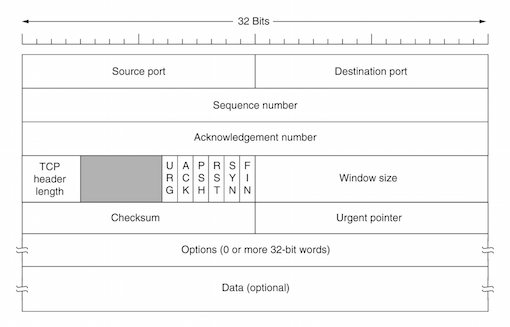
\includegraphics[width=\textwidth]{img/tcp2.png}}
	\caption{Uspořádání TCP packetu}
	\label{fig:tcp-packet}
\end{figure}

%\begin{figure}[H]
%    \centering
%	\makebox[\textwidth]{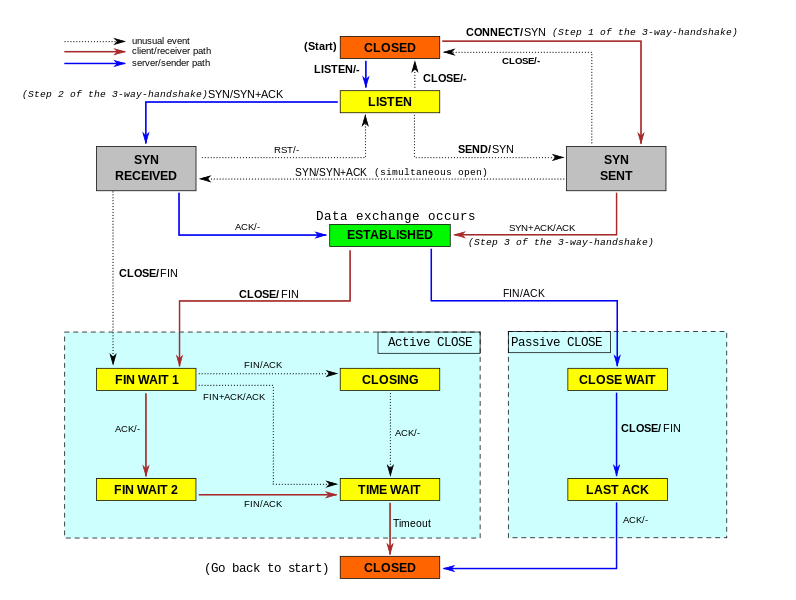
\includegraphics[width=\textwidth]{img/tcp.png}}
%	\caption{TCP stavový diagram}
%	\url{http://commons.wikimedia.org/wiki/File:Tcp_state_diagram_fixed_new.svg}
%	\label{fig:tcp}
%\end{figure}

\section{UDP}
% http://serverfault.com/questions/8981/what-is-the-difference-between-udp-and-tcp
fire and forget

\begin{figure}[h]
    \centering
	\makebox[\textwidth]{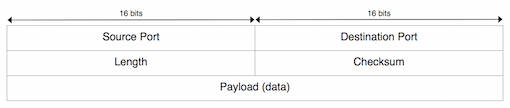
\includegraphics[width=\textwidth]{img/udp.png}}
	\caption{Uspořádání UDP datagramu}
	\label{fig:tcp-packet}
\end{figure}
\chapter{Volba vhodné technologie}

\section{Prvky senzorické sítě}
\section{Real-time server}

\section{Databázový server}
\subsection{RESP protokol}

\section{Webová aplikace}
\chapter{Struktura programového řešení}

\section{Komunikace koncentrátor - server}
\begin{minted}[linenos,breaklines]{c}
/**
  * @brief  Configurates the network interface
  * @param  None
  * @retval None
  */
static void Netif_Config(void) {
	struct ip_addr ipaddr;
	struct ip_addr netmask;
	struct ip_addr gw;
	
	IP4_ADDR(&ipaddr, IP_ADDR0, IP_ADDR1, IP_ADDR2, IP_ADDR3);
	IP4_ADDR(&netmask, NETMASK_ADDR0, NETMASK_ADDR1 , NETMASK_ADDR2, NETMASK_ADDR3);
	IP4_ADDR(&gw, GW_ADDR0, GW_ADDR1, GW_ADDR2, GW_ADDR3);
	
	/* Add the network interface */
	netif_add(&gnetif, &ipaddr, &netmask, &gw, NULL, &ethernetif_init, &ethernet_input);
	
	/* Registers the default network interface */
  netif_set_default(&gnetif);
  
  if (netif_is_link_up(&gnetif)) {
    /* When the netif is fully configured this function must be called */
    netif_set_up(&gnetif);
  } else {
    /* When the netif link is down this function must be called */
    netif_set_down(&gnetif);
  }
  
  /* Set the link callback function, this function is called on change of link status*/
  netif_set_link_callback(&gnetif, ethernetif_update_config);
}
\end{minted}

\begin{minted}[linenos,breaklines]{js}
udpSocket.on('message', function (msg, rinfo) {
    sails.log.verbose(JSON.stringify(msg.toString()));
    //FIXME: not good!
    if (result = msg.toString().match(/\*[0-9]+([\r][\n])(\$[0-9]+\1([0-9a-z]+)\1)+/i)) { //RESP
        //redisClient.lpush('TEMP_000001:data', result[3]);
        //redisClient.ltrim('TEMP_000001:data', 0, 999);

        redisClient.lpush('TEMP_000002:data', result[3]);
        redisClient.ltrim('TEMP_000002:data', 0, 999);
    }
    var message = new Buffer('test');
    udpSocket.send(message, 0, message.length, rinfo.port, rinfo.address);
}).bind(sails.config.globals.UDP_PORT, function () {
    sails.log('Starting UDP server (port ' + sails.config.globals.UDP_PORT + ')...');
});
\end{minted}

\section{Komunikace server - webová aplikace}
\chapter{Praktická aplikace}
Vzhled a ovládání celé aplikace je velmi jednoduché a intuitivní. Na úvodní stránce je přehled všech zařízení zapojených do sítě včetně jejich stavu. Vedle názvu zařízení je vidět, jestli je online, či nikoliv. Pod názvem je vidět aktuální přijatá informace v číselné podobě. Následuje seznam připojených a připojitelných zařízení. Jedním kliknutím je možné propojit jakékoliv koncentrátory. V tu chvíli začne server přeposílat příchozí data na všechna připojená zařízení. Počet připojitelných zařízení není nijak omezen. Toto je velká výhoda celého projektu. Není totiž vázán na fyzická spojení a příchozí data je tak možné poslat všem v síti bez dalších technických komplikací.

\begin{figure}[h]
    \centering
	\makebox[\textwidth]{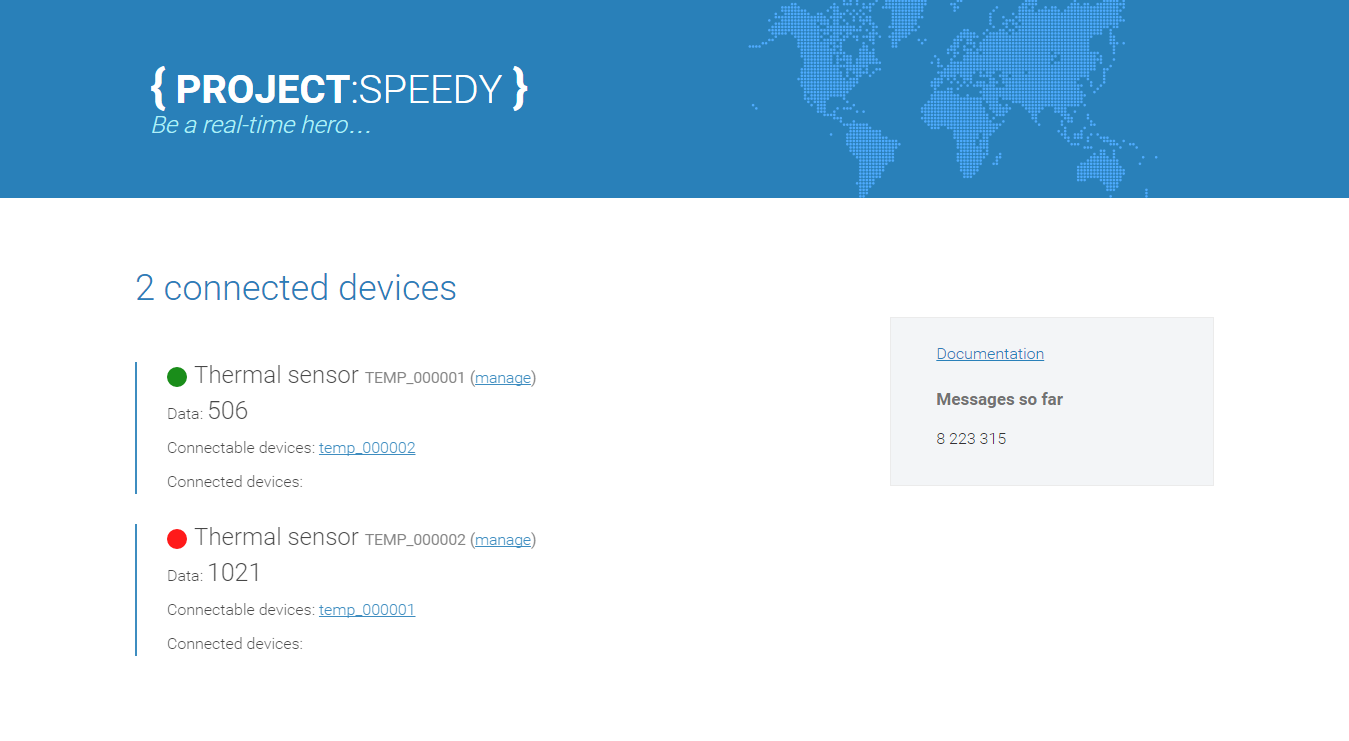
\includegraphics[width=\textwidth]{img/speedy1.png}}
	\caption{Úvodní stránka aplikace - přehled připojených zařízení}
	\label{fig:speedy1}
\end{figure}

Detail konkrétního zařízení poskytuje podobný pohled, navíc však ukazuje dodatečné informace jako jsou například IP adresy, nebo čas posledního ohlášení. Kromě samotné vizualizace historie příchozích dat je možné nastavit charakter dat odchozích. To znamená, že když bude připojeno další zařízení, nebudou se data rovnou přeposílat, ale najde se příslušná hodnota podle zvolené funkce a tato hodnota se pošle. Ve výchozím stavu se vše chová lineárně, tzn. jaká informace přijde, taková se přeposílá. Je však možné zvolit exponenciální viz rovnice \ref{eq:exp}, logaritmický (\ref{eq:log}), nebo vlnitý charakter (\ref{eq:vlna}). Poslední variantou je boolean závislost, kdy do hodnoty 512 včetně je výstupem 0, jinak maximální hodnota. Lze ji tedy definovat jako upravenou Heavisideovu funkci viz \ref{eq:bool}.

\begin{equation}
	y_{\_exp} = 1.80753 \cdot 1.00625^x
	\label{eq:exp}
\end{equation}

\begin{equation}
	y_{\_log} = -1053.96 + 289.931 \cdot ln(x)
	\label{eq:log}
\end{equation}

\begin{multline}
	y_{\_vlna} = -3.23206 \cdot 10^{-8} \cdot x^4 + 0.000068 \cdot x^3 - 0.044362 \cdot x^2 + \\
				+9.59513 \cdot x - 47.9076
	\label{eq:vlna}
\end{multline}

\begin{equation}
	y_{\_bool} = \left\{
		\begin{matrix}
			0 & \mbox{ pro }x \leq 512 \\
			1023 & \mbox{ pro }x > 512
		\end{matrix}
	\right.
	\label{eq:bool}
\end{equation}

Tyto funkce jsou naprogramovány ve složce \texttt{api/services} v souboru \texttt{FunctionsService.js}. Ukázková implementace logaritmické funkce vypadá takto:

\begin{minted}[linenos,breaklines]{js}
logarithmic: function (device, after_callback) {
  RedisService.del(device + ':table');
  for (var iterator = 0; iterator <= 1023; iterator++) {
    var entry = -1053.96 + (289.931 * (Math.log(iterator) / Math.log(Math.exp(1))));
    entry = entry <= 0 ? 0 : entry;
    entry = entry >= 1023 ? 1023 : entry;
    RedisService.hmset(device + ':table', iterator, Math.round(entry));
  }
  after_callback();
},
\end{minted}

Funkce tedy nejdříve maže předchozí převodní tabulku a následně ukládá nové vypočtené hodnoty. Pomocí ternárního operátoru \cite{ternar} jsou pak implementovány omezovače hodnot.

\begin{figure}[h]
	\begin{tikzpicture}
		\begin{axis}[width=0.95\textwidth,height=0.7\textwidth,xlabel={Vstupní hodnoty},ylabel={Výstupní hodnoty},legend style={at={(0.99,0.15)},anchor=east},grid=major]
			\addplot[red,domain=0:1024,samples=10]{x};
			\addlegendentry{Linerání závislost}
			\addplot[blue,domain=0:1024,samples=100]{1.80753*(1.00625^x)};
			\addlegendentry{Exponenciální závislost}
			\addplot[orange,domain=0:1024,samples=100]{-1053.96+(289.931*(ln(x)))};
			\addlegendentry{Logaritmická závislost}
			\addplot[purple,domain=0:1024,samples=200]{(-0.0000000323206*x^4)+(0.000068*x^3)+(-0.044362*x^2)+(9.59513*x)-47.9076};
			\addlegendentry{Vlnitá závislost}
	    \end{axis}
	\end{tikzpicture}
	\caption{Převodní funkce vstupních hodnot}
\end{figure}

Cílem této ukázky je ještě jednou znázornit, že celý systém pracuje na základě přeposílání jasně daných informací, které jsou realizovány pomocí jednoduchých čísel. Je tak možné provádět jakékoliv matematické operace bez nutnosti znalosti významu této informace. Tento přístup však není i\-de\-ál\-ní. V první řadě se až postupem času ukázalo, že rozsah 1024 hodnot je pro určité případy malý. To se projevuje například u rychlých výstupů (například diody). I při nejpomalejších změnách hodnot jsou tyto kroky rozpoznatelné. Jedná se o nepatrné změny, jsou však postřehnutelné. A to tím více, čím je nárůst hodnot strmější, tedy jak moc velká chyba vzniká v převodní tabulce. Jedno z možných řešení je zjemnění celého rozsahu, nebo neumožnění velkých skokových změn například pomocí některého z druhů klouzavého průměru. Je však zapotřebí myslet na to, že i tyto úpravy mají své nevýhody. V prvním případě množství hodnot a stále větší kmitání kolem jedné hodnoty, v druhém případě zpomalení systému.

Jedním z možných vylepšení je tak dvojité chování serveru. Ten by totiž mohl přijímat jak převedené hodnoty, tak obecné hodnoty z čidla. Server by jim sice nemohl rozumět (pokud by neměl sám implementovanou převodní tabulku), ale mohl by informaci přeposílat dále do sítě. Tato funkce v současné době není implementovaná a to hlavně z toho důvodu, že je náročné tyto informace nějakým způsobem využívat a skladovat v databázi, protože se jedná o velmi konkrétní problémy vázané na konkrétního výrobce zařízení, nebo čidla. Oproti tomu číselná interpretace hodnot dobře ukazuje, co je v této síti možné vytvořit.

\begin{figure}[h]
    \centering
	\makebox[\textwidth]{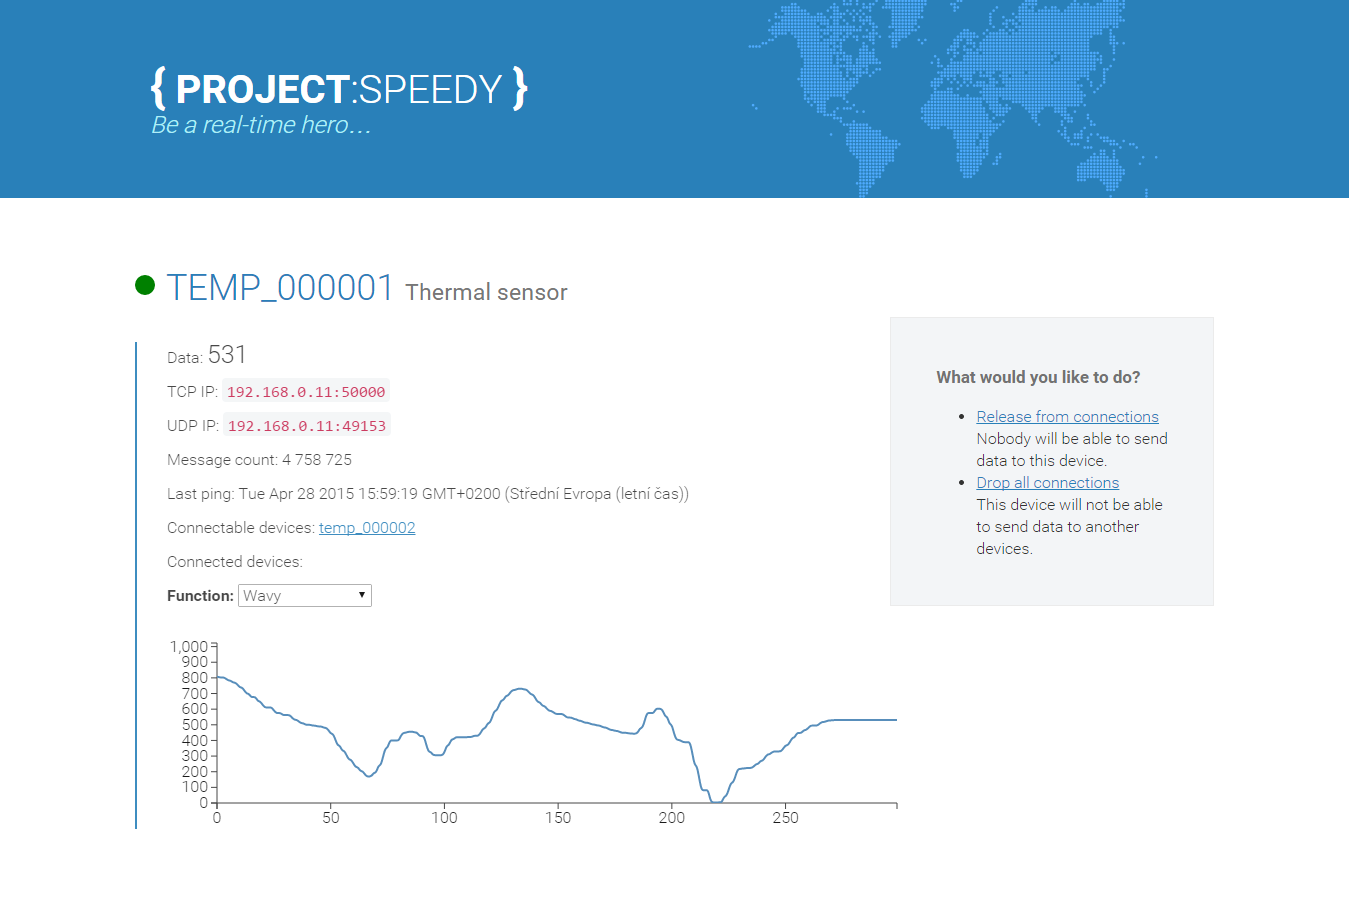
\includegraphics[width=\textwidth]{img/speedy2.png}}
	\caption{Detailní pohled na připojené zařízení}
	\label{fig:speedy2}
\end{figure}

Vzhledem ke svým vlastnostem je možné tuto síť použít jako domovní síť pro ovládání běžných prvků, což byl prvotní účel. Z hlediska technologie však tato síť není limitována pouze na ovládání elektroinstalace, ale je možné ji využít pro jakoukoliv senzorickou síť pro sběr dat a zároveň ovládání koncových členů. Její rozumné využití by bylo však tam, kde se bude struktura sítě často měnit, nebo zařízení přesouvat.

\chapter{Rozšíření stávajícího řešení}
Stávající řešení je plně funkční a splňuje veškeré požadavky v zadání. Jedná se však pouze o základ na kterém lze stavět systém, který by bylo možné použít v reálných budovách. Prvně je totiž zapotřebí tuto síť zabezpečit. To se týká zejména okamžiku, kdy by síť začala komunikovat přes Wi-Fi \index{Wi-Fi} (nebo jinou bezdrátovou technologii), ale platí to stejně i pro metalické vedení. Nesmí být možné, aby mohl kdokoliv ovlivňovat chování sítě, pokud k tomu není oprávněn.

Jak bylo již řečeno, samotná myšlenka není nijak limitována na přenos informace pomocí vodičů a je možné použít bezdrátovou komunikaci. Jednou ze zajímavých způsobů bezdrátové komunikace, ačkoliv také možná poněkud futuristickým, je Li-Fi \cite{lifi}. \index{Li-Fi} Tuto komunikaci poprvé představil prof. Harald Haas v roce 2011 v Edinburghu při vystoupení na konferenci TEDGlobal \cite{ted}. Jedná se o přenos informace pomocí viditelného světla. Tento přístup má celou řadu výhod. Kromě kapacity a efektivnosti stojí za zmínku hlavně fakt, že každý v budovách svítí a je tedy pro tento přenos informací vlastně připraven. V neposlední řadě se jedná o bezpečný přenos a to jak z hlediska lidského zdraví, tak i z hlediska různých nežádoucích odposlechů, protože se informace šíří pouze tam, kam dané světlo svítí (nikoliv např. skrz zeď). Síla a dosah signálu jsou tedy doslova vidět.

Dalším důležitým prvkem je implementace IPv6. \index{IPv6} Tyto adresy je možné využívat již od verze 1.4.x LwIP odděleně. V pozdějších verzích by mělo být možné použití IPv4 a IPV6 současně. \index{LwIP} V současné chvíli je totiž nepsaným předpokladem, že budou koncentrátory připojeny v privátní síti a využívají IPv4. \index{IPv4} Pokud by však měla síť fungovat i na veřejné síti, vzroste počet potřebných IP adres a již v tuto chvíli je jich nedostatek. Oproti tomu je IPv6 adres je $2^{128}$ \cite{ripe}\footnote{Ve skutečnosti je jich o něco méně viz článek od Chris Welsh \uv{Just how many IPv6 addresses are there? Really?} (\url{http://bit.ly/1Js6EpZ)}}, což je více než dostatek. V tomto projektu je použit LwIP stack, který IPv6 podporuje. Tato vlastnost není implementována, protože není potřeba. Pokud by se však projekt rozrostl do větších rozměrů, bylo by jej vhodné směřovat do stavu tzv. \uv{fog computingu}. \index{Fog computing} To znamená, že se z původně převážně centralizovaného systému začne stávat silně distribuovaný a původně centralizovaná část sítě bude sloužit pouze pro analýzy a statistiky. Veškeré zpracování dat se bude odehrávat na krajích sítě. Tím se vyřeší například problém s latencí. Zde by již bylo krátkozraké uvažovat překlad IP adres v rámci intranetové sítě, protože jednotlivými koncovými členy sítě mohou být jakákoliv připojitelná zařízení, tedy například automobily, mobilní senzory atd. Vzhledem k tomu, že je v současné chvíli celá síť závislá na centrálním serveru, nelze tento požadavek jednoduše implementovat. Bylo by však vhodné, aby se server začal postupně přesouvat na samotné koncentrátory, až by jej vůbec nebylo potřeba. To by znamenalo server úplně horizontálně rozškálovat, což v současnou chvíli není možné. Jednak proto, že by se to z hlediska Node.js \index{Node.js} nedělalo dobře, jednak také proto, že koncentrátory mají poměrně malý výkon. Malý výkon v tom smyslu, že pro rozumné spuštění Node.js, nebo konkurenčního io.js je nutné Linuxové prostředí. Nicméně reálně fungující projekt využívající OpenWrt Linux \cite{openwrt} s io.js je například Tessel 2 (Cortex\texttrademark-M3 CPU - 180 MHz) \cite{tessel}. \index{Tessel} Tento krok by přiblížil celý projekt k naprosto autonomní síti, kde by se velmi jednoduše řešil například výpadek jednoho z koncentrátorů. Přestala by totiž fungovat pouze malá část sítě. Navíc by bylo možné částečně se zbavit metalických vodičů a vytvářet tzv. mesh sítě, což by ostatně bylo žádoucí. Každý koncentrátor by se mohl bez větší námahy připojit na všechny koncentrátory, které jsou poblíž.

Dále je zajímavou myšlenkou implementovat real-time přenos i na komunikaci mezi koncentrátory a serverem např. Ethernet Powerlink. \index{Ethernet Powerlink} Tato vlastnost nebyla implementována ze dvou důvodů. Jednak to nebylo vzhledem k zadání žádoucí a dále při konzultaci se zadávající firmou byl stanoven závěr, že by tato náročná implementace neměla tak velký dopad, aby stálo za to real-time komunikaci v tomto slova smyslu řešit. V závěru práce se však ukazuje, že by jakákoliv real-time komunikace byla přínosem. Celý systém totiž sice funguje, ale není nijak časově závislý. To není uživatelsky přívětivé. V současné chvíli také není implementováno ani přijímání adres z DHCP serveru, kvůli jednoduchosti. Na funkcionalitě se nic nemění, je však možné pohodlně vyvíjet, bez nutnosti dalšího prvku v síti.

V neposlední řadě bude také nutné vybavit síť velkým počtem růz\-no\-ro\-dých prvků jako jsou různé vypínače, snímače a akční členy, protože dobrou síť dělá mimo jiného také počet možností, které lze se sítí dělat.

\chapter{Závěr}

%TODO shrnutí výsledků
%TODO říct, že je možné metalická i bezdrátová síť
%TODO nedostatky, technická omezení
%TODO konfrontace zadání (vytyčených cílů)
%TODO doporučení pro další autorem navrhovaný postup, řešení, úpravy, které nebylo možné např. z časových důvodů zrealizovat





\begin{thebibliography}{99}
\addcontentsline{toc}{chapter}{Literatura}
%http://www.citace.com/

\bibitem{rfc6455}
FETTE, Ian a Alexey MELNIKOV. The WebSocket Protocol. \textit{The Internet Engineering Task Force} [online]. 2011 [cit. 2015-05-20]. Dostupné z: \url{https://tools.ietf.org/html/rfc6455}

\bibitem{real-time}
LAMMERMANN, Sebastian. Ethernet as a Real-Time Technology. \textit{Lammermann.eu} [online]. 2008 [cit. 2015-05-20]. Dostupné z: \url{http://www.lammermann.eu/wb/media/documents/real-time_ethernet.pdf}

\bibitem{mistrovstvi}
SOSINSKY, Barrie A. \textit{Mistrovství – počítačové sítě}. Vyd.~1. Brno: Computer Press, 2011, 840~s. Mistrovství (Computer Press). ISBN 978-80-251-3363-7. 

\bibitem{cube}
\textit{Getting started with STM32CubeF2 firmware package for STM32F2xx series: User manual} [online]. 2014 [cit. 2015-05-20]. Dostupné z: \url{http://www.st.com/st-web-ui/static/active/en/resource/technical/document/user_manual/DM00111485.pdf}

\bibitem{nodejs}
\textit{Node.js} [online]. [cit. 2015-05-20]. Dostupné z: \url{http://nodejs.org/}

\bibitem{redis}
\textit{Redis.io} [online]. [cit. 2015-05-20]. Dostupné z: \url{http://redis.io/}

\bibitem{redis-cluster}
Redis cluster tutorial. \textit{Redis.io} [online]. 2015 [cit. 2015-05-20]. Dostupné z: \url{http://redis.io/topics/cluster-tutorial}

\bibitem{redis-benchmark}
How fast is Redis?. \textit{Redis.io} [online]. [cit. 2015-05-20]. Dostupné z: \url{http://redis.io/topics/benchmarks}

\bibitem{hal}
\textit{Description of STM32F4xx HAL drivers: User manual} [online]. 2015 [cit. 2015-05-20]. Dostupné z: \url{http://www.st.com/st-web-ui/static/active/en/resource/technical/document/user_manual/DM00105879.pdf}

\bibitem{manual}
\textit{Reference manual - STM32F405xx/07xx, STM32F415xx/17xx, STM32F42xxx and STM32F43xxx advanced ARM\textregistered-based 32-bit MCUs} [online]. 2015 [cit. 2015-05-20]. Dostupné z: \url{http://www.st.com/web/en/resource/technical/document/reference_manual/DM00031020.pdf}

\bibitem{icmp}
POSTEL, Jon. Internet Control Message Protocol. \textit{The Internet Engineering Task Force} [online]. 1981 [cit. 2015-05-27]. Dostupné z: \url{http://tools.ietf.org/html/rfc792}

\bibitem{sails}
\textit{Sails.js} [online]. [cit. 2015-05-20]. Dostupné z: \url{http://sailsjs.org/}

\bibitem{ripe}
Understanding IP Addressing. \textit{RIPE NCC} [online]. [cit. 2015-05-20]. Dostupné z: \url{http://bit.ly/1JvOvaO}

\bibitem{openwrt}
Linux distribution for embedded devices. \textit{OpenWrt} [online]. [cit. 2015-05-20]. Dostupné z: \url{https://openwrt.org/}

\bibitem{tessel}
\textit{Tessel 2} [online]. [cit. 2015-05-20]. Dostupné z: \url{https://tessel.io/}

\bibitem{cluster}
Node.js v0.12.3 Manual \& Documentation. \textit{Cluster} [online]. [cit. 2015-05-20]. Dostupné z: \url{https://nodejs.org/api/cluster.html}

\bibitem{v8}
\textit{V8 JavaScript Engine} [online]. [cit. 2015-05-20]. Dostupné z: \url{https://code.google.com/p/v8/}

\bibitem{heroku}
\textit{Heroku} [online]. [cit. 2015-05-20]. Dostupné z: \url{https://www.heroku.com/}

\bibitem{forever}
A~simple CLI tool for ensuring that a given script runs continuously. \textit{Forever} [online]. [cit. 2015-05-20]. Dostupné z: \url{https://github.com/foreverjs/forever}

\bibitem{q}
A~tool for creating and composing asynchronous promises in JavaScript. \textit{Q} [online]. [cit. 2015-05-20]. Dostupné z: \url{http://documentup.com/kriskowal/q/}

\bibitem{socket}
\textit{Socket.IO} [online]. [cit. 2015-05-20]. Dostupné z: \url{http://socket.io/}

\bibitem{cordova}
Platform for building native mobile applications using HTML, CSS and JavaScript. \textit{Apache Cordova} [online]. [cit. 2015-05-20]. Dostupné z: \url{http://cordova.apache.org/}

\bibitem{meteor}
Running your app on Android or iOS. \textit{Meteor} [online]. [cit. 2015-05-20]. Dostupné z: \url{https://www.meteor.com/try/7}

\bibitem{lifi}
\textit{pureLiFi} [online]. [cit. 2015-05-20]. Dostupné z: \url{http://purelifi.com/}

\bibitem{ternar}
VRÁNA, Jakub. \textit{1001 tipů a triků pro PHP}. Vyd.~1. Brno: Computer Press, 2010, 136 Co je ternární operátor. ISBN 978-80-251-2940-1.

\bibitem{ted}
prof. HAAS, Harald. Wireless data from every light bulb. \textit{TED - Ideas worth spreading} [online]. 2011 [cit. 2015-05-20]. Dostupné z: \url{http://www.ted.com/talks/harald_haas_wireless_data_from_every_light_bulb}

\end{thebibliography}

\addcontentsline{toc}{chapter}{Rejstřík}
\printindex

\end{document}